\section{Scelte di Progettazione} % presentiamo il codice
Nella seguente sezione verranno trattati le principali scelte di progettazione atte all'analisi dei dati delle matrici e ai corrispettivi dati riscontrati dall'analisi. La figura \ref{fig:Progettazione} mostra i passi fondamentali eseguiti durante tutta la durata della sperimentazione:
\begin{enumerate}
    \item Esecuzione del metodo di Cholesky sulle singole Matrici al variare dell'OS e del linguaggio.
    \item Salvataggio dei dati riscontrati.
    \item Analisi dei dati.
\end{enumerate}
\begin{figure}[h!]
    \centering
    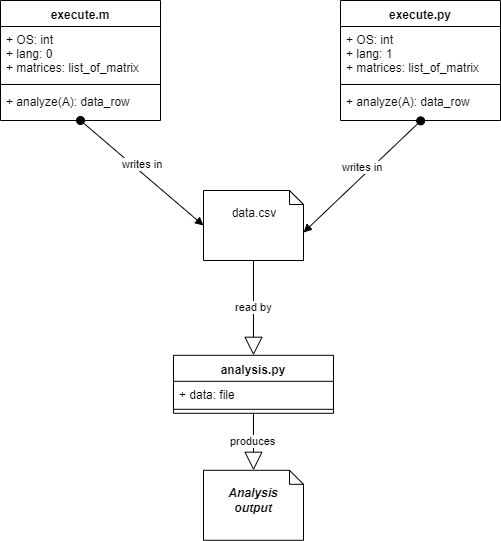
\includegraphics[width=0.5\textwidth]{figs/Structure Flowchart.png}
    \caption{Diagramma UML di progettazione}
    \label{fig:Progettazione}
\end{figure}
La seguente trattazione non ha il compito di definire in modo particolarmente tecnico tutta la fase di progettazione, bensi' si vuole soffermare su quegli aspetti ritenuti fondamentali per comprendere al meglio l'operato. Dalla figura \ref{fig:Progettazione} si possono notare anche molteplici altri aspetti:
\begin{enumerate}
    \item \textbf{Reperimento Dati:} sono stati utilizzati due script (\textit{execute.m} e \textit{execute.py}) per eseguire il metodo di Cholesky sulle varie matrici e per il reperimento dei corrispettivi dati. E' doveroso sottolineare che essi non hanno il compito di analizzare i dati da essi stessi prodotti. L'utilizzo di questa metodologia ha permesso una migliore divisione tra le componenti adibite al reperimento dei dati e quelle per la corrispettiva analisi. 
    Un approccio diverso sarebbe stato estramamente lento e poco preciso per una corretta e omogenea analisi.
    \item \textbf{Salvataggio Dati:} il salvataggio dei dati, riscontrati al punti precedente, avviene mediante un file \textit{data.csv} che verrà analizzato come se fosse un \textbf{dataset}.
    \item \textbf{Analisi dei Dati:} l'analisi dei dati è stata effettuata a posteriori rispetto al reperimento dati, in particolar modo dopo aver eseguito i due script sui sistemi operativi di interesse. Questa procedura ha permesso di analizzare i dati in maniera indipendente rispetto agli script atti al reperimento dei dati.
\end{enumerate}
Nelle prossime sezioni verranno trattati più in dettaglio i procedimenti sfruttati e le librerie utilizzate per lo scopo. Oltre a ciò verrà anche definita l'architettura sfruttata per l'esecuzione dei diversi Sistemi Operativi.
\subsection{L'utilizzo della Virtualizzazione}
Al fine di garantire una più pulita analisi dei dati si è optato per l'utilizzo della virtualizzazione dei sistemi Linux e Microsoft Windows, su cui si sono svolti i dovuti test. In particolare la scelta in ambiente linux si è rivolta sulla distribuzione \textbf{\href{https://lubuntu.me/}{Linux Lubuntu}}, mentre in ambiente Microfost Windows la scelta è ricaduta su \textbf{\href{https://www.microsoft.com/it-it/software-download/windows10}{Windows 10}}.
\paragraph{HyperVisor} Per favorire la miglior virtualizzazione possibile è stato necessario l'impiego dell'hypervisor~(\cite{itwiki:120906467}) che è il componente centrale e più importante di un sistema basato sulle macchine virtuali. Un computer sul quale venga eseguito un hypervisor che a sua volta controlla una o più macchine virtuali è detto macchina host, e ogni macchina virtuale è detta macchina guest. Il compito di un hypervisor è quello di presentare all'utente i sistemi operativi delle macchine guest e di gestire la loro esecuzione. Grazie ad un hypervisor, su una macchina host possono essere in esecuzione contemporaneamente diverse macchine guest, su ognuna delle quali può girare un sistema operativo diverso che ha il controllo sulle risorse hardware virtualizzate rese disponibili dall'hypervisor. La ragione per cui è stato scelto è inerente al fatto che questo tipo di virtualizzazione è diversa dalla virtualizzazione a livello di sistema operativo, dove tutte le istanze (dette anche container) devono essere eseguite in un unico kernel. \\
In particolar modo è opportuno sottolineare che per tale scopo è stato sfruttato \textbf{\href{https://docs.microsoft.com/it-it/virtualization/hyper-v-on-windows/about/}{Microsoft Hyper-V}}, ovvero un \textbf{HyperVisor di tipo 1} (\textit{native hypervisor}). Questa tipologia di virtualizzazione offre numerosi benefici rispetto agli \textbf{HyperVisor di tipo 2} (\textit{hosted hypervisor}). Sebbene in questa esposizione non si voglia entrare nel merito della questione, nella figura \ref{fig:HyperVisor} sono schematizzate le principali differenze tra i due sistemi di virtualizzazione. \\
è doveroso sottolineare che la virtualizzazione è stata eseguita sfruttando lo stesso \textit{hardware} per entrambi i sistemi operativi testati, in particolare ad ognuno di essi sono stati dedicati 6 core sulla CPU (\textit{Intel(R) Core(TM) i7-10710U CPU @ 1.10GHz 1.61 GHz}) e 8GB di RAM.
\begin{figure}[h!]
    \centering
    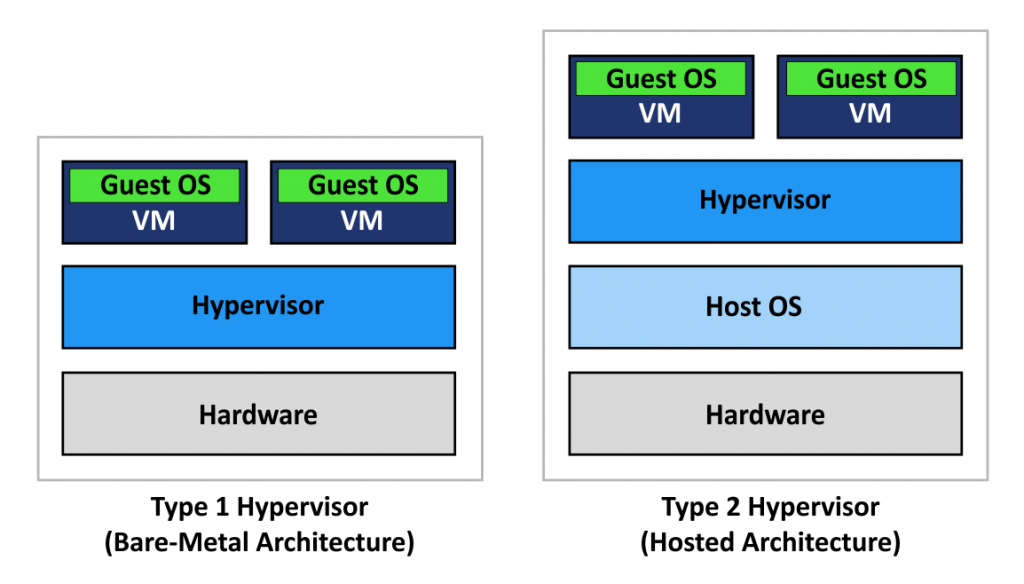
\includegraphics[width=1\textwidth]{figs/Type-1-and-type-2-hypervisor-1024x584.png}
    \caption{HyperVisor Types from \href{https://www.nakivo.com/blog/it/hyper-v-virtualbox-one-choose-infrastructure-2/}{www.nakivo.com}}
    \label{fig:HyperVisor}
\end{figure}

\section{Reperimento Dati}
Questa sezione ha il compito di introdurre più in dettaglio le strutture di progettazione (e i 
\subsubsection{Matlab}
\myworries{Come ho fatto il matlab? Puoi usare lstinputlisting per inserire codice matlab (già gestito da me nella sintassi di latex) }

\paragraph{Problemi Riscontrati e limitazioni}
\myworries{Problematiche riscontrate? Backslash funziona?}

\subsubsection{Python}
Per gestire al meglio la giusta separazione tra gli elementi del progetto si è deciso di sfruttare un particolare pattern strutturale definito dallo schema sottostante. Il modello, cattura il comportamento dell'applicazione in termini di dominio del problema e gestisce direttamente i dati, la logica e le regole del progetto. \\ Nella seguente trattazione, al fine di evitare panoramiche fuori focus, si vogliono sottolineare solo gli aspetti fondamentali utilizzati per il reperimento dei dati tramite l'esecuzione del metodo di Choleksy.


\begin{forest}
  for tree={
    font=\ttfamily,
    grow'=0,
    child anchor=west,
    parent anchor=south,
    anchor=west,
    calign=first,
    edge path={
      \noexpand\path [draw, \forestoption{edge}]
      (!u.south west) +(7.5pt,0) |- node[fill,inner sep=1.25pt] {} (.child anchor)\forestoption{edge label};
    },
    before typesetting nodes={
      if n=1
        {insert before={[,phantom]}}
        {}
    },
    fit=band,
    before computing xy={l=15pt},
  }
[PythonProject
   [src
      [Analyze
          [\_\_init\_\_.py]
          [analyze.py]
          [helper.py]
      ]
      [Model
          [\_\_init\_\_.py]
          [execute.py]
          [helper.py]
      ]
      [\_\_init\_\_.py]
      [costants.py]
    ]
]
\end{forest}\\

\paragraph{Lo script execute.py}
Lo script \textit{execute.py} svolge il ruolo primario dell'intero ecosistema python. Esso ha il compito di prendere in considerazione ogni matrice per poi analizzarla singolarmente mediante lo script \textit{analyze.py}. La figura \ref{fig:execute.py} ne mostra il funzionamento.
\begin{figure}[h!]
    \centering
    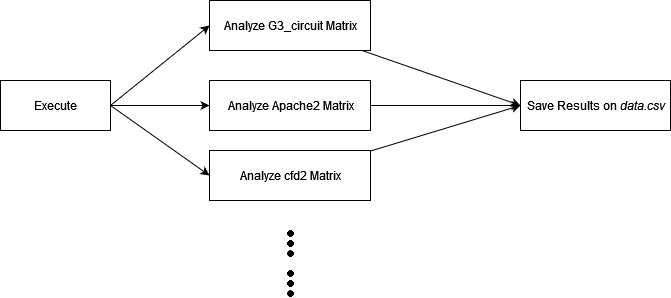
\includegraphics[width=0.7\textwidth]{figs/execute.drawio.png}
    \caption{Funzionamento dello script \textit{execute.py}}
    \label{fig:execute.py}
\end{figure}

\paragraph{Lo script analyze.py}
Il package \textbf{Analyze} si occupa principalmente di andare ad applicare ad una spefica matrice il metodo di \textbf{Cholesky}. Il codice \ref{AnalyzeClass} riporta l'implementazione della classe fondamentale situata nel file \textbf{analyze.py}.

\lstinputlisting[language=Python, caption= Analyze Class, label=AnalyzeClass]{CODE/Py/Analyze.py}

Come si può notare essa racchiude le parti fondamentali dell'operazione effettuata, in particolar modo si vuole sottolineare l'importanza della funzione \textbf{\_\_analyze(self, path)}. Essa prevede in input il \textit{path} dov'è situata la matrice da leggere. La funzione esegue i seguenti step:
\begin{enumerate}
    \item Lettura della Matrice
    \item Inizio dell'analisi sulla memoria occupata e sul tempo impiegato.
    \item Esecuzione del metodo di Cholesky
    \item Fine dell'analisi sulla memoria occupata e sul tempo impiegato.
    \item Calcolo dell'errore relativo rispetto alla soluzione fornita di default.
\end{enumerate}
Come si può facilmente notare dal codice \ref{AnalyzeClass}, si è predisposto il tutto per scrivere i risultati ottenuti in tabelle \textit{*.csv}, al fine di facilitarne l'analisi futura.

\paragraph{L'utilizzo di \textit{Scikit-Sparse}}
Python fornisce librerie di default per trattare matrici con il metodo di Cholesky, tra esse è doveroso nominare \textbf{Numpy}~(\cite{harris2020array}) e \textbf{SciPy}~(\cite{2020SciPy-NMeth}). Sfortunatamente queste librerie non foniscono un metodo diretto per analizzare \textbf{matrici sparse}, per cui la scelta è ricaduta su una libreria \textbf{open-source} chiamata \textbf{\href{https://scikit-sparse.readthedocs.io/en/latest/}{Scikit-Sparse}}. Essa si basa su \textit{SciPy.Sparse} ma, al contrario di quest'ultima, offre funzioni veloci ed efficienti per trattare matrici sparse con Cholesky. Il codice \ref{scikitsparsecholesky} mostra l'implementazione effettuata tramite l'utilizzo della libreria sopra indicata. Si noti che tale funzione viene richiamata dal metodo \_\_analyze(self, path) a riga \textit{21}.

\lstinputlisting[language=Python, caption= scikit\_sparse\_cholesky function, label=scikitsparsecholesky]{CODE/Py/scikitSparse.py}

\paragraph{Problemi Riscontrati e limitazioni}
La principale problematica, riscontrata durante la progettazione dell'ecosistema Python, ricade principalmente nella struttura della libreria utilizzata. Sfortunatamente la compilazione di \textit{Scikit-Sparse} non fornisce esito positivo in ambienti \textbf{Microsoft Windows}. I test sono stati effettuati mediante l'ausilio del package manager \href{https://pypi.org/project/pip/}{Pip} e \href{https://www.anaconda.com/products/distribution}{Anaconda}, ma nessuno ha dato buon fine. Per questo motivo si è ritenuto opportuno l'utilizzo della \textbf{WSL} (\textit{Windows Subsystem for Linux}) al fine di risolvere la problematica.
\subsection{Salvataggio Dati}
\myworries{Qui inseriamo il dataset prodotto}

\subsection{Analisi Dei Dati}
Nella seguente sottosezione verranno trattate le procedure di progettazione utilizzate durante l'analisi dei dati prodotti, in particolare le librerie utilizzate. In particolare i dati analizzati saranno quelli provenienti dai file \textit{*.csv}. Per far ciò è stato sfruttato \textit{JupyterBook} \cite{perez2011python} mediante il linguaggio Python. Di seguito viene proposta la struttura dell'intero progetto di analisi.\\
\begin{forest}
  for tree={
    font=\ttfamily,
    grow'=0,
    child anchor=west,
    parent anchor=south,
    anchor=west,
    calign=first,
    edge path={
      \noexpand\path [draw, \forestoption{edge}]
      (!u.south west) +(7.5pt,0) |- node[fill,inner sep=1.25pt] {} (.child anchor)\forestoption{edge label};
    },
    before typesetting nodes={
      if n=1
        {insert before={[,phantom]}}
        {}
    },
    fit=band,
    before computing xy={l=15pt},
  }
[PythonAnalysis
   [src
      [model
          [\_\_init\_\_.py]
          [additional\_analysis.ipynb]
          [backslash\_comparison.ipynb]
          [LanguageCompare.ipynb]
          [OSCompare.ipynb]
      ]
      [Resources
          [data.csv]
          [dataBackslash.csv]
      ]
    ]
]
\end{forest}\\
Si noti che l'analisi è stata volutamente strutturata in diverse sotto-analisi:
\begin{itemize}
    \item Analisi dei Linauggi
    \item Analisi degli OS
    \item Confronto metodo \textit{Chol} con \textit{Backslash} in Matlab
    \item Analisi aggiuntive e di interesse
\end{itemize}
\subsubsection{Librerie utilizzate}
Le librerie sfruttate allo scopo sono molteplici, ma si vuole sottolineare l'importanza di \textit{matplotlib} \cite{Hunter:2007} e \textit{pandas} \cite{reback2020pandas} \cite{mckinney-proc-scipy-2010}. Allo scopo sono state realizzate delle funzioni per la creazione \textbf{omogenea} di tutti i grafici utilizzati durante l'analisi.  Il codice \ref{plot} ne fornisce un esempio implementativo.

\lstinputlisting[language=Python, caption= Plot functions, label=plot]{CODE/Py/plot.py}